\chapter{OCM Sound Generator}

\section{Problem}

Das Oldenburger Computer-Museum (OCM) verfolgt das Ziel, Besucherinnen und Besuchern
die Entwicklung historischer Computersysteme möglichst praxisnah zu vermitteln. Viele
Ausstellungsstücke können direkt bedient werden und ermöglichen dadurch einen
interaktiven Einblick in die Funktionsweise früher Computersysteme. Ein Bereich, der im
Museum bislang jedoch nur wenig behandelt wird, ist die Erzeugung von Tönen und
Geräuschen auf historischen Heimcomputern.

Gerade frühe Computer verfügten nur über sehr begrenzte Hardware-Ressourcen. Dennoch
gelang es Entwicklerinnen und Entwicklern bereits in den 1970er- und 1980er-Jahren,
Musik, Soundeffekte und sogar einfache Sprachausgaben zu erzeugen. Diese technische
Entwicklung stellt einen wichtigen Bestandteil der Computergeschichte dar und eignet sich
besonders gut für eine interaktive Museumsanwendung.

Ziel unseres Projektes war es daher, Besucherinnen und Besuchern die Grundlagen der
digitalen Klangerzeugung näherzubringen und gleichzeitig die Unterschiede zwischen
historischen Computersystemen verständlich zu machen. Dabei sollte die Anwendung nicht
nur Informationen vermitteln, sondern den gesamten Entstehungsprozess eines Sounds
interaktiv erfahrbar machen.

\section{Idee}

Zu Beginn des Projektes wurden verschiedene Lösungsansätze entwickelt und hinsichtlich
ihrer Umsetzbarkeit bewertet.

Der erste Ansatz bestand darin, den im vorherigen Semester entwickelten
dreidimensionalen Synthesizer weiterzuentwickeln. Ziel war es zunächst, das bereits
modellierte Instrument spielbar zu machen. Nach mehreren Diskussionen innerhalb der
Gruppe zeigte sich jedoch, dass dieser Ansatz gegenüber bereits existierenden
Web-Synthesizern keinen ausreichenden Mehrwert bieten würde. Gleichzeitig hätte die
dreidimensionale Bedienung die Benutzung eher erschwert als verbessert. Aus diesem
Grund wurde dieser Ansatz verworfen.

Als zweite Idee entstand ein Soundwellen-Visualisierer. Hierbei sollten unterschiedliche
Signalformen wie Sinus-, Rechteck-, Dreieck- oder Sägezahnwellen sowohl akustisch als
auch grafisch dargestellt werden. Dieser Ansatz überzeugte zwar durch seine gute
Veranschaulichung der verschiedenen Signalformen, erschien jedoch für den geplanten
Projektumfang zu eingeschränkt.

Schließlich entwickelte sich aus beiden Ideen das endgültige Konzept des
\textbf{OCM Sound Generators}. Die Anwendung verbindet die grafische Darstellung von
Wellenformen mit einer interaktiven Erstellung eigener Soundsequenzen. Besucherinnen
und Besucher können dabei mehrere aufeinanderfolgende Sounds erzeugen, verändern und
anschließend auf historischen Computersystemen wiedergeben.

\section{Projekt}

Im Rahmen des Projektes entstand eine vollständig webbasierte Anwendung zur
Erstellung einfacher Retro-Soundsequenzen. Innerhalb der Anwendung können bis zu fünf
aufeinanderfolgende Schritte erzeugt werden. Jeder Schritt besteht aus mehreren
gleichzeitig abgespielten Tönen, deren Frequenz, Lautstärke, Dauer und Wellenform frei
eingestellt werden können. Zusätzlich kann jeder Schritt um unterschiedliche
Rauschgeneratoren ergänzt werden.

Ein wesentliches Merkmal der Anwendung ist die unmittelbare grafische Darstellung der
erzeugten Schallwellen. Änderungen an den Parametern werden sofort sowohl akustisch
als auch visuell sichtbar, wodurch ein direkter Zusammenhang zwischen Eingabe und
Klangerzeugung entsteht.

Die eigentliche Audioausgabe erfolgt vollständig innerhalb des Webbrowsers mithilfe der
Web Audio API. Dadurch ist keine zusätzliche Softwareinstallation erforderlich und die
Anwendung kann auf unterschiedlichen Endgeräten verwendet werden. Neben klassischen
Rechtecksignalen können auch verschiedene Rauschtypen erzeugt werden, welche typische
Klangeffekte historischer Heimcomputer simulieren.

Nach Fertigstellung einer Soundsequenz kann die Anwendung sämtliche Parameter in
einer kompakten Zeichenkette speichern und daraus automatisch einen QR-Code
erzeugen. Durch das Scannen dieses QR-Codes gelangen Besucherinnen und Besucher auf
eine zweite Webanwendung. Dort werden sämtliche Sounddaten wieder eingelesen und in
BASIC-Code für unterschiedliche historische Computersysteme übersetzt.

Aktuell unterstützt die Anwendung den Commodore 64 sowie den TI-99/4A. Die erzeugten
Programme können anschließend direkt an den entsprechenden Museumsrechnern
eingegeben und ausgeführt werden. Dadurch erleben Besucherinnen und Besucher den
vollständigen Weg von der Erstellung eines Sounds bis zur Wiedergabe auf originaler
historischer Hardware.

Während der Entwicklung wurde besonderer Wert auf eine modulare Architektur gelegt.
Neue Computersysteme können später durch zusätzliche Exportmodule ergänzt werden,
ohne dass die eigentliche Soundgenerierung verändert werden muss. Dadurch bleibt das
Projekt langfristig erweiterbar und kann flexibel an zukünftige Anforderungen des
Oldenburger Computer-Museums angepasst werden.

\section{Aufgabenteilung}

Die Entwicklung des Projektes erfolgte arbeitsteilig innerhalb unseres Teams. Die
Aufgaben wurden entsprechend der individuellen Interessen und vorhandenen
Vorkenntnisse verteilt.

\begin{table}[H]
\centering
\begin{tabular}{|p{3.5cm}|p{10cm}|}
\hline
\textbf{Name} & \textbf{Aufgaben} \\ \hline
Engin Budak &
Dokumentation, Recherche, Projektidee \\ \hline

Fyn Paajanen &
Konzeption und Entwicklung des physischen Prototyps,
Recherche im Bereich Mikrocontroller,
Entwurf des Controllergehäuses,
Dokumentation \\ \hline

Markus Vogel &
Implementierung der Webanwendung,
Weiterentwicklung der Funktionen,
Dokumentation \\ \hline

Maximilian Goldmann &
UI/UX-Design,
Attraction-Mode,
Implementierung der Benutzeroberfläche \\ \hline

\end{tabular}
\caption{Aufgabenverteilung innerhalb des Projektes}
\end{table}

\section{Physischer Prototyp}

Neben der webbasierten Anwendung entstand die Idee, den Besucherinnen und Besuchern
eine physische Eingabemöglichkeit bereitzustellen. Ziel war es, die Bedienung intuitiver
zu gestalten und gleichzeitig den Bezug zu historischen Computersystemen zu stärken.
Anstatt sämtliche Eingaben ausschließlich über Maus oder Touchscreen vorzunehmen,
sollte die Anwendung über einen speziell entwickelten Controller gesteuert werden.

Der Controller orientiert sich an klassischen Bedienkonzepten früher Computertechnik.
Dadurch entsteht eine haptische Interaktion, welche die eigentliche Anwendung sinnvoll
ergänzt und den Museumsbesuch interaktiver gestaltet.

\subsection{Hardware}

Als technische Grundlage wurde ein ESP32-Mikrocontroller ausgewählt. Der ESP32
vereint einen leistungsfähigen Mikrocontroller mit integriertem WLAN und Bluetooth auf
einem einzigen Entwicklungsboard und eignet sich dadurch besonders gut für interaktive
Projekte mit Webanbindung.

Für den ersten Funktionsprototyp wurde ein Breadboard verwendet. Dieses ermöglicht
einen schnellen und flexiblen Aufbau elektronischer Schaltungen, ohne dass bereits eine
eigene Leiterplatte gefertigt werden muss. Dadurch konnten unterschiedliche
Schaltungskonzepte getestet und einzelne Komponenten unkompliziert ausgetauscht
werden.

Der Hardware-Prototyp besteht aus folgenden Komponenten:

\begin{table}[H]
\centering
\begin{tabular}{|p{5cm}|p{9cm}|}
\hline
\textbf{Komponente} & \textbf{Funktion} \\ \hline
ESP32 &
Steuerung des gesamten Controllers und Kommunikation mit der Webanwendung \\ \hline

Drehencoder &
Veränderung der Frequenz des aktuell ausgewählten Tons \\ \hline

Druckfunktion des Drehencoders &
Auslösen zusätzlicher Bedienfunktionen \\ \hline

Taster 1 &
Starten der Wiedergabe (Play) \\ \hline

Taster 2 &
Stoppen der Wiedergabe (Stop) \\ \hline

Taster 3 &
Erzeugen des QR-Codes beziehungsweise Druckfunktion (Print) \\ \hline

Breadboard &
Prototypischer Aufbau der Hardware \\ \hline
\end{tabular}
\caption{Verwendete Hardwarekomponenten}
\end{table}

Der Drehencoder bildet das zentrale Eingabeelement des Controllers. Im Gegensatz zu
einem herkömmlichen Potentiometer besitzt dieser keinen festen Anschlag und kann
beliebig oft in beide Richtungen gedreht werden. Dadurch eignet er sich besonders gut
für kontinuierliche Parameter wie die Veränderung einer Frequenz.

Zusätzlich verfügt der Encoder über eine integrierte Druckfunktion, wodurch weitere
Bedienaktionen umgesetzt werden können, ohne zusätzliche Hardware einsetzen zu
müssen.

\subsection{Kommunikation zwischen Controller und Webanwendung}

Der ESP32 verarbeitet sämtliche Eingaben der angeschlossenen Bedienelemente lokal.
Sobald der Benutzer einen Taster betätigt oder den Drehencoder bewegt, werden diese
Ereignisse unmittelbar vom Mikrocontroller erkannt.

Über die integrierte WLAN-Schnittstelle können die erfassten Eingaben anschließend an
die Angular-Webanwendung übertragen werden. Dort werden die empfangenen Daten
verarbeitet und direkt auf die Benutzeroberfläche angewendet. Änderungen der
Frequenz werden beispielsweise unmittelbar sowohl grafisch in der
Wellenformdarstellung als auch akustisch innerhalb der Soundausgabe sichtbar.

Die Kommunikation wurde bewusst drahtlos vorgesehen. Dadurch muss der Controller
nicht dauerhaft per USB mit dem Anzeigerechner verbunden sein und kann flexibel in
eine spätere Museumsinstallation integriert werden. Gleichzeitig ermöglicht diese
Architektur zukünftige Erweiterungen, beispielsweise mehrere Controller oder weitere
interaktive Eingabegeräte.

Die prototypische Umsetzung konzentrierte sich zunächst auf die grundlegende
Funktionsfähigkeit der Hardware. Ziel war es, zunächst die zuverlässige Erfassung der
Benutzereingaben sicherzustellen, bevor eine vollständige Integration in die
Webanwendung erfolgt.

\begin{figure}[H]
    \centering
    \begin{tikzpicture}[
    node distance=2.2cm,
    every node/.style={draw, rounded corners, align=center, minimum width=3.8cm, minimum height=1cm},
    >=Stealth
    ]
    
    \node (user) {Besucher};
    \node (controller) [below=of user] {OCM Sound Controller\\ESP32};
    \node (web) [below=of controller] {Angular\\Webanwendung};
    \node (output) [below=of web] {Audioausgabe\\Wellenform\\QR-Code};
    
    \draw[->] (user) -- (controller);
    \draw[->] (controller) -- node[right]{WLAN} (web);
    \draw[->] (web) -- (output);
    
    \end{tikzpicture}
    \caption{Kommunikation zwischen dem physischen Controller und der Webanwendung.}
    \label{fig:kommunikation}
    \end{figure}

    Abbildung~\ref{fig:kommunikation} verdeutlicht den geplanten Informationsfluss
zwischen dem physischen Controller und der Webanwendung. Die Bedienung erfolgt
zunächst über den OCM Sound Controller, der auf einem ESP32-Mikrocontroller basiert.
Drehbewegungen des Encoders sowie das Betätigen der Taster werden vom ESP32
erfasst und verarbeitet. Anschließend werden die entsprechenden Informationen über
die integrierte WLAN-Schnittstelle an die Webanwendung übertragen.

Die Angular-Anwendung verarbeitet diese Eingaben unmittelbar und aktualisiert die
jeweiligen Parameter der Soundgenerierung. Änderungen an der Frequenz oder
Steuerbefehle wie das Starten oder Stoppen der Wiedergabe wirken sich dadurch
direkt auf die grafische Wellenformdarstellung sowie die erzeugte Audioausgabe aus.
Die klare Trennung zwischen Eingabegerät und Anwendung ermöglicht eine flexible
Erweiterung des Systems und vereinfacht die spätere Integration in den Museumsbetrieb.

\subsection{Gehäusekonzept}

Nachdem die grundlegende Funktionalität der Hardware auf dem Breadboard erfolgreich
umgesetzt werden konnte, wurde ein Konzept für ein eigenes Controllergehäuse
entwickelt. Ziel war es, sämtliche elektronischen Komponenten in einem kompakten
Gehäuse unterzubringen und den Besucherinnen und Besuchern eine intuitive
Bedienoberfläche bereitzustellen.

Der Controller sollte bewusst schlicht gestaltet werden, um den Fokus auf die
Interaktion mit der Anwendung zu legen. Gleichzeitig orientiert sich das Design an der
Bedienlogik historischer Computerhardware. Der Drehencoder befindet sich im oberen
Bereich des Gehäuses und dient als zentrales Eingabeelement zur Veränderung der
Frequenz. Im unteren Bereich befinden sich drei Drucktaster für die wichtigsten
Steuerfunktionen der Anwendung.

Die Frontplatte sollte mithilfe von vier Schrauben befestigt werden. Dadurch lässt sich
das Gehäuse jederzeit öffnen und vereinfacht sowohl Wartungsarbeiten als auch den
Austausch einzelner Komponenten. Der ESP32 sollte im Inneren des Gehäuses befestigt
werden, wodurch sämtliche Kabel geschützt verlaufen und von außen nicht sichtbar
sind.

Die nachfolgenden Skizzen zeigen das geplante Konzept des Controllers.

\begin{figure}[H]
    \centering
    \includegraphics[width=0.75\textwidth]{bilder/controller_front.jpeg}
    \caption{Konzeptskizze der Vorderseite des Controllers mit Drehencoder und Funktionstasten.}
    \label{fig:controller_front}
\end{figure}

Die Vorderseite wurde so entworfen, dass alle wichtigen Bedienelemente gut erreichbar
sind. Der große Abstand zwischen Drehencoder und Tastern verhindert Fehlbedienungen
und ermöglicht eine komfortable Nutzung auch über einen längeren Zeitraum.

\begin{figure}[H]
    \centering
    \includegraphics[width=0.70\textwidth]{bilder/controller_side.jpeg}
    \caption{Seitliche Schnittdarstellung des geplanten Controllergehäuses.}
    \label{fig:controller_side}
\end{figure}

Die Seitenansicht verdeutlicht den geplanten inneren Aufbau des Controllers. Der ESP32
wird im Gehäuse befestigt und über kurze Leitungen mit den Bedienelementen verbunden.
Dadurch entsteht ein kompakter Aufbau, der sich problemlos transportieren und später
im Museum einsetzen lässt.

\subsection{Erster Hardware-Prototyp}

Vor der Entwicklung eines endgültigen Gehäuses wurde zunächst ein vollständiger
Funktionsprototyp auf einem Breadboard aufgebaut. Dieser diente dazu, sämtliche
Komponenten zu testen und die Kommunikation zwischen Hardware und Software
schrittweise zu entwickeln.

\begin{figure}[H]
    \centering
    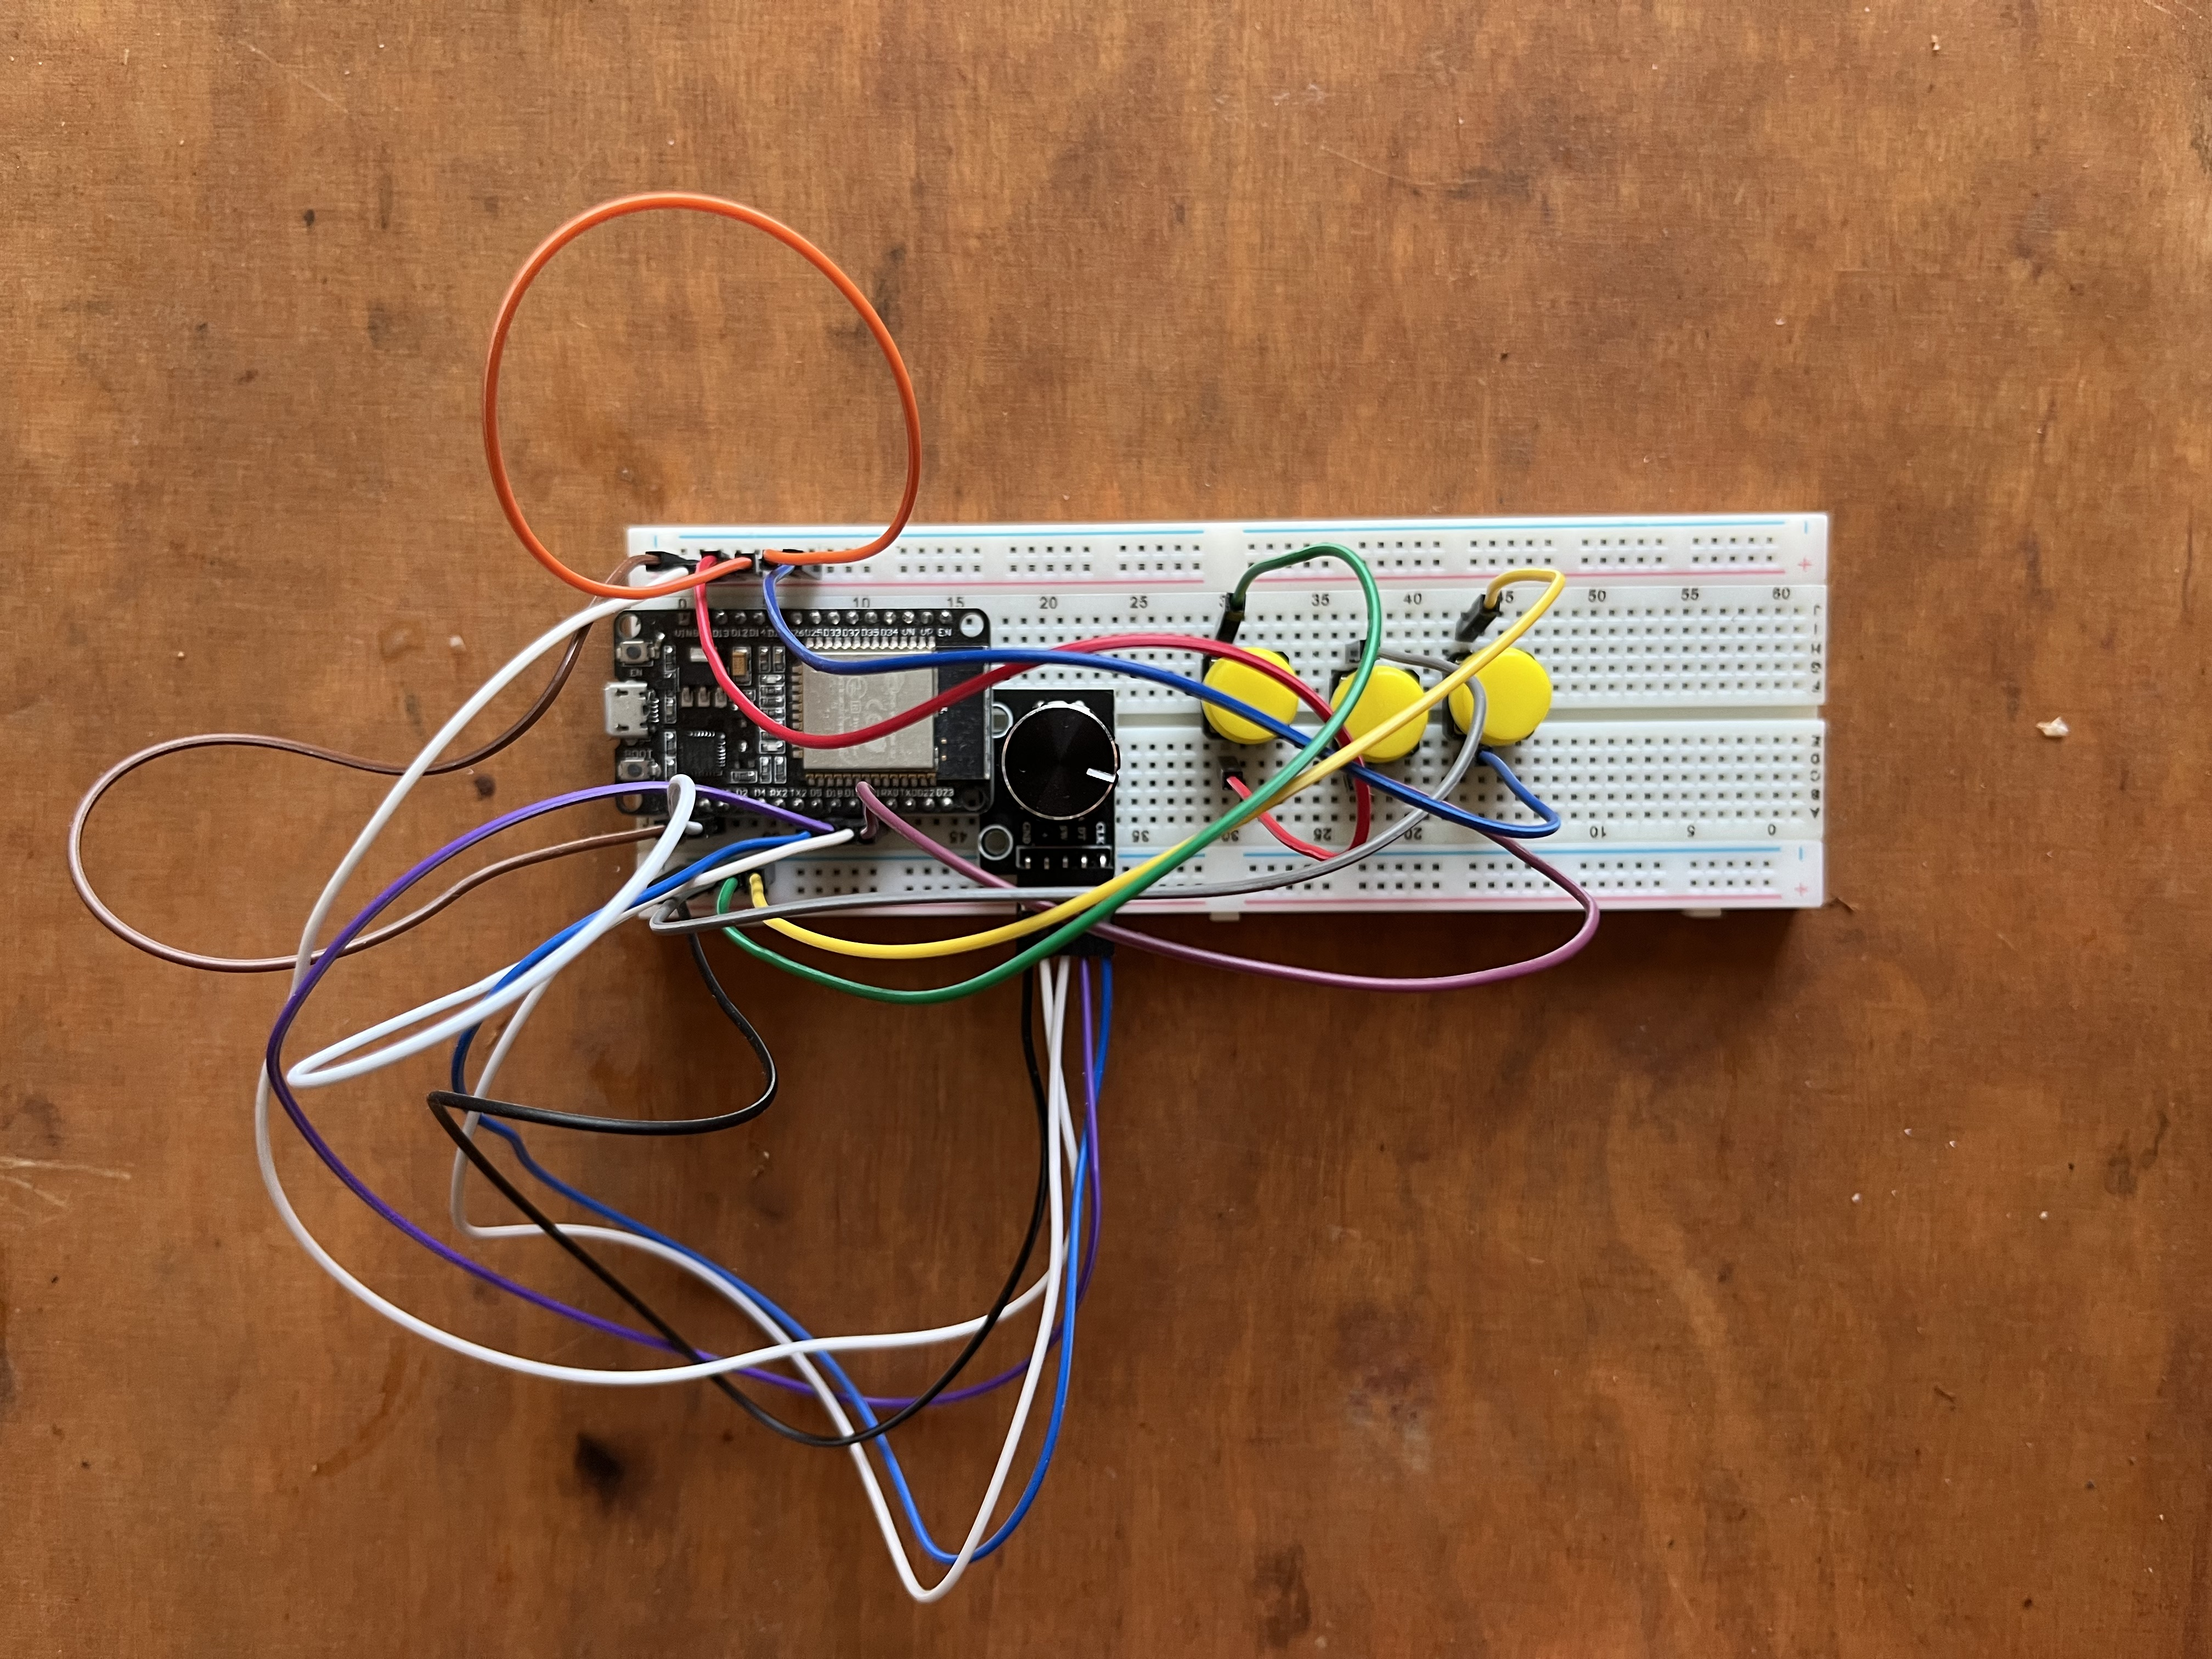
\includegraphics[width=0.60\textwidth]{bilder/hardware_prototype.jpeg}
    \caption{Erster Hardware-Prototyp mit ESP32, Breadboard, Drehencoder und Tastern.}
    \label{fig:prototype}
\end{figure}

Der Aufbau besteht aus einem ESP32-Entwicklungsboard, einem inkrementellen
Drehencoder sowie drei Drucktastern. Alle Komponenten wurden zunächst auf einem
Breadboard verbunden, wodurch Änderungen an der Schaltung jederzeit ohne großen
Aufwand möglich waren.

Während der Entwicklung konnten bereits sämtliche Eingabeelemente erfolgreich
angesprochen werden. Der ESP32 erkannte sowohl die Betätigung der Taster als auch
die Drehrichtung des Encoders zuverlässig. Damit wurde die technische Grundlage für
eine spätere Anbindung an die Webanwendung geschaffen.

Der Aufbau diente ausschließlich als Entwicklungsplattform und war nicht für den
dauerhaften Einsatz vorgesehen. Im weiteren Projektverlauf sollte die Elektronik
anschließend in das entwickelte Gehäuse integriert und durch eine kompaktere
Leiterplattenlösung ersetzt werden.

\section{Technische Anleitung}

Zum Testen der Anwendung wird lediglich das Projekt
\texttt{xr-museum-server-main} benötigt.

Nach dem Installieren der Abhängigkeiten mittels

\begin{verbatim}
npm install
\end{verbatim}

kann die Anwendung mit

\begin{verbatim}
npm start
\end{verbatim}

oder alternativ

\begin{verbatim}
npx ng serve
\end{verbatim}

gestartet werden.

Die Anwendung ist anschließend unter

\begin{center}
\texttt{http://localhost:4200}
\end{center}

im Browser erreichbar.

\section{Fazit}

Im Verlauf des Projektes konnten zahlreiche neue Kenntnisse in den Bereichen
Webentwicklung, Audioprogrammierung und Mikrocontrollertechnik erworben werden.
Insbesondere die Kombination aus einer webbasierten Anwendung und einem physischen
Controller stellte eine interessante Erweiterung des ursprünglichen Projektumfangs dar.

Obwohl der Hardware-Prototyp aufgrund des begrenzten Zeitrahmens nicht vollständig
fertiggestellt werden konnte, wurde ein funktionsfähiger Demonstrator entwickelt und ein
vollständiges Gehäusekonzept ausgearbeitet. Die grundlegende technische Machbarkeit
konnte damit erfolgreich nachgewiesen werden.

Für zukünftige Arbeiten bietet das Konzept zahlreiche Erweiterungsmöglichkeiten.
Hierzu gehören unter anderem die Entwicklung einer eigenen Leiterplatte, die Fertigung
des Gehäuses mittels 3D-Druck sowie die vollständige Integration der Hardware in die
Webanwendung. Dadurch könnte Besucherinnen und Besuchern des Oldenburger
Computer-Museums künftig eine noch interaktivere Möglichkeit zur Erzeugung und
Steuerung historischer Computersounds angeboten werden.

\section{Weiterentwicklung}

Der entwickelte Hardwareaufbau stellt einen ersten funktionsfähigen
Machbarkeitsnachweis für den geplanten Museumscontroller dar. Im Rahmen des
Projekts lag der Schwerpunkt zunächst auf der Erprobung der einzelnen Komponenten
sowie auf der Entwicklung eines geeigneten Bedienkonzepts. Die erfolgreiche
Ansteuerung des Drehencoders und der Taster sowie die geplante Kommunikation mit
der Webanwendung zeigen, dass die technische Umsetzung grundsätzlich möglich ist.

Für eine zukünftige Weiterentwicklung ist vorgesehen, den aktuellen Breadboard-Aufbau
durch eine eigens entwickelte Leiterplatte (PCB) zu ersetzen. Dadurch können die
elektrischen Verbindungen dauerhaft ausgeführt und die Zuverlässigkeit des Systems
erhöht werden. Gleichzeitig würde sich der Platzbedarf der Elektronik deutlich
verringern.

Darüber hinaus soll das entworfene Controllergehäuse mittels 3D-Druck gefertigt
werden. Dadurch können sämtliche Komponenten sicher im Inneren des Gehäuses
untergebracht werden, während die Bedienelemente ergonomisch auf der Frontseite
angeordnet bleiben. Das Gehäuse schützt die Elektronik vor äußeren Einflüssen und
ermöglicht gleichzeitig einen einfachen Zugang für Wartungs- oder Reparaturarbeiten.

Langfristig soll der Controller vollständig mit der Webanwendung gekoppelt werden,
sodass Besucherinnen und Besucher sämtliche Funktionen der Soundgenerierung
direkt über die physische Hardware bedienen können. Dadurch entsteht eine
authentischere und interaktivere Benutzererfahrung, welche den Museumsbesuch
zusätzlich aufwertet.